\documentclass{article}
\usepackage[utf8]{inputenc}
\usepackage{bm}
\usepackage{../../lib/approx-scribe}

\usepackage{todonotes}


\begin{document}
\lecture{4}{Submodular Maximization Part 1}{Antares Chen}{3/6/2019}

A submodular function is a function that models diminishing returns. Many problems such as min-cut, maxcut, Max-SAT, and maximal matching can be formulated as maximizing an appropriate submodular function. In the proceeding two notes, we conclude our discussion of greedy approximation algorithms by discussing algorithms for maximizing submodular functions. We begin by studying the problem of maximizing a \emph{monotone} submodular function under cardinality constraints. We discuss a $\big( 1 - \frac{1}{e} \big)$-approximation algorithm due to Cornuejols, Fisher, and Nemhauser~\cite{CFN77}.

\section{Two Motivating Problems}

Let us consider two problems which will motivate our study of monotone submodular functions.

\subsection{Maximizing Float Among Bank Accounts}

Prior to the days of electronic checking, one could accrue money through interest during the time between when a check is first issued, and when it is cashed. This amount of time is called \emph{float} and it was often advantageous for companies to maintain multiple bank accounts in order to maximize float and thus interest gained. In a practice called \emph{check kiting}, a particularly clever individual, or business, could scam a number banking institutions by issuing a check from a deficient checking account, and cover the deficit via a check from another account with insufficient funds. The individual can continue issuing checks from deficient accounts each to cover the previously issued check while still accruing interest on the money in each account\footnote{On a completely unrelated note, UGTCS does not condone bank fraud.}.

We model the problem of maximizing float in the following manner. We are given a collection of bank institutions $\mathcal{B}$ and individuals $\mathcal{P}$ for which we need to make regular payments to. For each $i \in \mathcal{B}$ and $j \in \mathcal{P}$, the amount of float for writing a check from bank $i$ to payee $j$ is given by $\nu_{ij}$. Given $k > 0$, our goal is to pick $k$ banks to open accounts at such that the total amount of float gained from paying each individual is maximized. More precisely, we wish to choose $S \subseteq \mathcal{B}$ such that
\begin{equation*}
f(S) = \sum_{j \in \mathcal{P}} \max_{i \in S} \nu_{ij}
\end{equation*}

is maximized.

\subsection{Maximizing Social Influence}

With the advent of massive social networks such as Instagram, Snapchat, and Twitter, individuals with a large enough social following can categorize themselves as \emph{social media influencers}. A particular marketing strategy for product companies (used quite frequently in markets such as beauty, gaming, and electronics) involves sponsoring social influencers with free products in exchange for advertisement in their social media postings. In theory, influencers are provided steady support for their lifestyles while the product company increases their notoriety amongst the influencers's followers. Given that a particular social network could have many influencers, each with followers from different demographics, it is advantageous for product companies to appropriately choose subsets of influencers to sponsor in order to maximize their influence on target groups.

Kempe, Kleinberg, and Tardos proposes a model for this scenario in the following sense. We are given a social network $G = (V, E)$ where each vertex is associated with a binary state of either being ``influenced'' or not. Each vertex $v \in V$ is associated with a \emph{activation threshold} $\theta_v \in [0, 1]$ such that $v$ only becomes \emph{influenced} if $\theta_v$ fraction of its neighbors are influenced. Given $k > 0$, the problem of \emph{maximizing the spread of social influence} is the task of choosing an initial subset of $k$ ``influenced'' vertices $S \subseteq V$ which maximize the number of vertices that will eventually become influenced.

\section{Submodular Functions}

What do these two problems have in common? Each can be formulated as searching for a subset of elements, subject to a \emph{cardinality constraint}, that maximizes a cost function where the cost function is \emph{submodular}. Let us now define submodular functions.

\begin{definition}
Let $E = [n]$ be a set of elements, and $f: 2^E \rightarrow \mathbb{R}_{\geq 0}$ a function on subsets $S \subseteq E$ such that $f(\varnothing) = 0$. $f$ is submodular if and only if for all $S, T \subseteq E$ where $S \subseteq T$ and $\ell \notin T$, we have
\begin{equation}\label{eqn:submodular-def-1}
f(T \cup \{ \ell \}) - f(T) \leq f(S \cup \{ \ell \}) - f(S)
\end{equation}
\end{definition}

Equivalently, we can also define submodularity via

\begin{definition}
A function $f: 2^E \rightarrow \mathbb{R}_{\geq 0}$ is submodular if and only if for all $S, T \subseteq E$, we have
\begin{equation}\label{eqn:submodular-def-2}
f(S \cup T) \leq f(S) + f(T) - f(S \cap T)
\end{equation}
\end{definition}

One way of thinking about submodular functions is that it models a notion of ``diminishing returns''. Notice that inequality~\ref{eqn:submodular-def-1} states that, for $S \subseteq T$, one gains less by adding $\ell$ to $T$ compared to adding $\ell$ to $S$. As more elements are added to the set of interest, the increase in cost decreases.

\begin{figure}[h!]
  \centering
  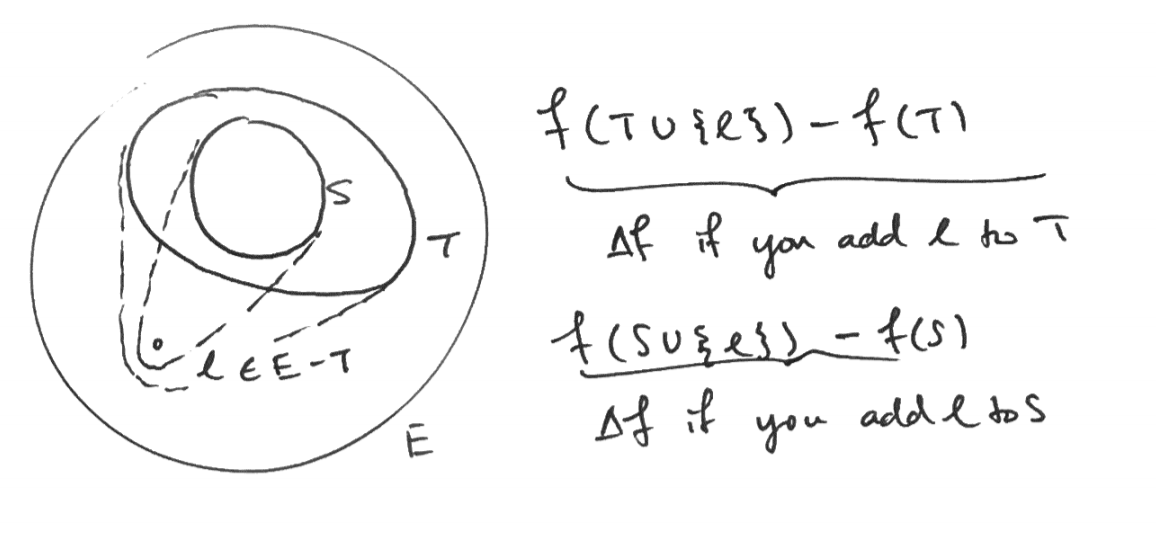
\includegraphics[scale=0.3192]{images/image-1.png}
\end{figure}

% A second interpretation is that submodularity captures a discretized analogue of convexity. If we have a function $f: X \rightarrow \mathbb{R}$ defined over a convex subset $X$ of (say) $\mathbb{R}^n$, then we would say $f$ is \emph{convex} if for all $x, y \in X$, the image of any point in the convex combination of $x$ and $y$ under $f$ is upperbounded by the convex combination of $f(x)$ and $f(y)$. That is to say for any $\lambda \in [0, 1]$ we have:
% \begin{equation*}
% f(\lambda x + (1 - \lambda) y) \leq \lambda f(x) + (1 - \lambda) f(y)
% \end{equation*}
%
% For submodular $f$, its domain is discrete. Inequality~\ref{eqn:submodular-def-2} considers the discrete analogue of convex combination to be the union of two subsets $S, T$ and the upperbound of its image under $f$ to be given by the inclusion-exclusion principle.

As an example, we note that the cost function for maximizing float is submodular.

\begin{claim}\label{claim:float-submodular}
The problem of maximizing float across multiple bank accounts maximizes a submodular function.
\end{claim}
\begin{proof}
Given a collection of banks $\mathcal{B}$, payees $\mathcal{P}$, and floats $\nu_{ij}$ between bank $i \in \mathcal{B}$ and payee $j \in \mathcal{P}$, consider the function $f: 2^\mathcal{B} \rightarrow \mathbb{R}_{\geq 0}$ defined via the following.
\begin{equation*}
f(S) = \sum_{j \in \mathcal{P}} \max_{i \in S} \nu_{ij}
\end{equation*}

It is immediate that $f(\varnothing) = 0$. Consider any $S \subseteq T \subseteq \mathcal{B}$ and $\ell \notin T$. For $S$, we have the following
\begin{equation*}
f(S \cup \{ \ell \}) - f(S)
= \sum_{j \in \mathcal{P}} \bigg( \max_{i \in S \cup \{ \ell \}} \nu_{ij} - \max_{i \in S} \nu_{ij} \bigg)
= \sum_{j \in \mathcal{P}} \max \bigg( 0, \nu_{\ell j} - \max_{i \in S} \nu_{ij} \bigg)
\end{equation*}

The last equality follows as for each term in the summand, $i$ for $\max_{i \in S \cup \{ \ell \}} \nu_{ij}$ can either be in $S$ or be $i = \ell$. Hence the difference will either be $0$ if $i \in S$ or $\nu_{\ell j} - \max_{i \in S} \nu_{ij}$ if $i = \ell$. By similar reasoning:
\begin{equation*}
f(T \cup \{ \ell \}) - f(T)
= \sum_{j \in \mathcal{P}} \max \bigg( 0, \nu_{\ell j} - \max_{i \in T} \nu_{ij} \bigg)
\end{equation*}

However, $S \subseteq T$ which means that $\max_{i \in T} \nu_{ij} \geq \max_{i \in S} \nu_{ij}$. This implies the following:
\begin{equation*}
f(T \cup \{ \ell \}) - f(T)
= \sum_{j \in \mathcal{P}} \max \bigg( 0, \nu_{\ell j} - \max_{i \in T} \nu_{ij} \bigg)
\leq \sum_{j \in \mathcal{P}} \max \bigg( 0, \nu_{\ell j} - \max_{i \in S} \nu_{ij} \bigg)
= f(S \cup \{ \ell \}) - f(S)
\end{equation*}

as required.
\end{proof}

\subsection{Monotonicity}

The cost functions for maximizing float and social influence benefit from the additional property of being \emph{monotone}. A submodular function $f: 2^E \rightarrow \mathbb{R}_{\geq 0}$ is monotone if for all $S, T \subseteq E$ such that $S \subseteq T$, we have
\begin{equation*}
f(S) \leq f(T)
\end{equation*}

As an example, we can demonstrate that the cost function for float maximization is monotone.
\begin{claim}
Maximizing float across multiple bank accounts maximizes a monotone submodular function.
\end{claim}
\begin{proof}
Proceeding from a similar calculation in claim~\ref{claim:float-submodular}, we note that
\begin{equation*}
f(T) - f(S)
= \sum_{j \in \mathcal{P}} \bigg( \max_{i \in T} \nu_{ij} - \max_{i \in S} \nu_{ij} \bigg)
= \sum_{j \in \mathcal{P}} \max \bigg( 0, \max_{i \in T - S} \nu_{ij} - \max_{i \in S} \nu_{ij} \bigg)
\geq 0
\end{equation*}

where last equality follows since $S \subseteq T$. We conclude that $f(T) \geq f(S)$.
\end{proof}

\section{A Greedy Approximation Algorithm}

Let us now precisely define the problem of maximizing a monotone submodular function subject to a cardinality constraint. Let $E = [n]$ be a ground set of elements and let $f: 2^E \rightarrow \mathbb{R}_{\geq 0}$ be a monotone submodular function. Given $k > 0$, we wish to find $S \subseteq E$ such that $\lvert S \rvert \leq k$ and $S$ maximizes $f(S)$. In general, this problem is $\NP$-hard as it reduces to set cover. For this reason, we seek an approximation algorithm. The greedy algorithm that we will now present is due to Cornuejols, Fisher, and Nemhauser~\cite{CFN77}.

The greedy approximation proceeds exactly how one would expect it to. Initialize the set $S = \varnothing$ and so long as $\lvert S \rvert \leq k$, add an element $i$ to $S$ that maximizes the gain in the cost function.

\noindent\fbox {
\parbox{45.5em} {
\textbf{Monotone Submodular Algorithm}

Given ground set $E$ and submodular function $f: 2^E \rightarrow \mathbb{R}_{\geq 0}$, initialize $S_0 = \varnothing$. Do for $t = 1, \ldots, k$:

\begin{quote}
\begin{enumerate}[1.]
\item Choose $i_t$ subject to the following
\begin{equation*}
i_t = \argmax_{i \in E} \Big( f(S_0 \cup \{ i \}) - f(S_0) \Big)
\end{equation*}

\item Update $S_t = S_{t-1} \cup \{ i_t \}$

\item Remove $E = E - \{ i_t \}$
\end{enumerate}
\end{quote}
}
}
\vspace{1em}

Our goal will be to demonstrate that $S_k$ returned by the algorithm above provides a $(1 - \frac{1}{e})$-approximation. The approximation ratio will follow directly from this lemma:

\begin{lemma}\label{lem:monotone-sub-mod}
Let $O \subseteq E$ be the optimal solution. Then for any iteration $t$ of the algorithm, the following holds for the remaining elements of $E$.
\begin{equation*}
\max_{i \in E} \Big( f(S_t \cup \{ i \}) - f(S_t) \Big) \geq \frac{1}{k} \big( f(O) - f(S) \big)
\end{equation*}
\end{lemma}

The lemma posits that for each iteration, there exists a choice that makes up a $k$-th fraction of the difference between the algorithm's current solution and the best solution. Why should we expect this to be true? Because not everyone can be \emph{below average} -- since $\lvert O \rvert \leq k$, there has to exist $i \in O \subseteq E$ such that $f(\{ i \}) \geq \frac{f(O)}{k}$. Elements are greedily added to $S$, meaning the first element $i_1$ added to $S$ must increase the value of $S$ by $\frac{f(O)}{k}$. Hypothetically, there then exists another element $i'$ such that $f(S \cup \{ i' \}) - f(S) \geq \frac{1}{k} (f(O) - f(S))$

Let us defer the proof of this lemma for now, and demonstrate the bound on the approximation ratio.

\begin{theorem}
The algorithm gives a $\big( 1 - \frac{1}{e} \big)$-approximation algorithm for the problem of maximizing a monotone submodular function.
\end{theorem}
\begin{proof}
With $S_k$ returned by the algorithm, we can compute $f(S_k)$ as follows:
\begin{equation*}
f(S_k) = f(S_{k-1} \cup \{ i_k \})
\end{equation*}

Because $i_t$'s are chosen greedily, lemma~\ref{lem:monotone-sub-mod} gives us
\begin{align*}
f(S_{k-1} \cup \{ i_k \})
&\geq \frac{1}{k} f(O) + \bigg( 1 - \frac{1}{k} \bigg) f(S_{k-1}) \\
&= \frac{1}{k} f(O) + \bigg( 1 - \frac{1}{k} \bigg) f(S_{k-2} \cup \{ i_{k-1}) \\
&\geq \frac{1}{k} f(O) + \bigg( 1 - \frac{1}{k} \bigg) \bigg( \frac{1}{k} f(O) + \bigg( 1 - \frac{1}{k} \bigg) f(S_{k-2}) \bigg) \\
&= \frac{1}{k} f(O) \bigg( 1 + \bigg( 1 - \frac{1}{k} \bigg) \bigg) + \bigg( 1 - \frac{1}{k} \bigg)^2 f(S_{k-2})
\end{align*}

Proceeding via this pattern, we derive the following
\begin{align*}
f(S_k)
&= \frac{1}{k} f(O) \bigg( 1 + \bigg( 1 - \frac{1}{k} \bigg) + \ldots + \bigg( 1 - \frac{1}{k} \bigg)^{k-1} \bigg) \\
&= \frac{1}{k} f(O) \sum_{i=0}^{k-1} \bigg( 1 - \frac{1}{k} \bigg)^i \\
&= \frac{1}{k} f(O) \frac{1 - (1 - 1/k)^k}{(1 - (1/k))} \\
&= f(O) \cdot \bigg( 1 - \bigg( 1 - \frac{1}{k} \bigg)^k \bigg)
\end{align*}

By the theoretician's favorite inequality, we have $1 - x \leq e^{-x}$ for all $x \geq 0$. Hence
\begin{equation*}
f(O) \bigg( 1 - \bigg( 1 - \frac{1}{k} \bigg)^k \bigg)
\geq f(O) \Big( 1 - \big( e^{-1/k} \big)^k \Big)
= f(O) \bigg( 1 - \frac{1}{e} \bigg)
\end{equation*}

We thus derive that $f(S_k) \geq f(O) \cdot (1 - \frac{1}{e})$ as required.
\end{proof}

Now to prove the lemma. Notice that the proceeding argument relies on a clever use of the definition for monotone submodularity.

\begin{proof}[Proof of lemma~\ref{lem:monotone-sub-mod}]
Observe that $O \subseteq O \cup S_t$ for any $t$. Thus by submodularity we have
\begin{equation*}
f(O) \leq f(O \cup S_t)
\end{equation*}

Let us annotate the items of $O$ as $O = \{ i_1^*, \ldots, i_p^* \}$ for some $p \leq k$. We write $f(O \cup S_t)$ as the following telescoping sum:
\begin{equation*}
f(O \cup S_t) = f(S_t) + \sum_{j=1}^p \Big( f(S_t \cup \{ i_1^*, \ldots, i_j^* \}) - f(S_t \cup \{ i_1^*, \ldots, i_{j-1}^*) \Big)
\end{equation*}

However, $S_t \subseteq S_t \cup \{ i_1^*, \ldots, i_{j-1}^* \}$ hence by submodularity, we have the following.
\begin{equation*}
f(S_t) + \sum_{j=1}^p \Big( f(S_t \cup \{ i_1^*, \ldots, i_j^* \}) - f(S_t \cup \{ i_1^*, \ldots, i_{j-1}^*) \Big)
\leq f(S_t) + \sum_{j=1}^p \Big( f(S_t \cup \{ i_j^* \} ) - f(S_t) \Big)
\end{equation*}

We can upperbound the sum by replacing each term with $f(S_t \cup \{ i' \}) - f(S_t)$ for maximal $i' \in E$ giving us
\begin{align*}
f(S_t) + \sum_{j=1}^p \Big( f(S_t \cup \{ i_j^* \} ) - f(S_t) \Big)
&\leq f(S_t) + p \cdot \max_{i \in E} \Big( f(S \cup \{ i \}) - f(S) \Big) \\
&\leq f(S_t) + k \cdot \max_{i \in E} \Big( f(S \cup \{ i \}) - f(S) \Big)
\end{align*}

We have $f(O)\leq f(S_t) + k \cdot \max_{i \in E} \big( f(S \cup \{ i \}) - f(S) \big)$ which is equivalent to the required claim.
\end{proof}

\section{Concluding Remarks}

In the next set of notes, we will discuss maximizing submodular functions when we are not provided cardinality constraints, nor guaranteed monotonicity.

\bibliographystyle{plain}
\begin{thebibliography}{99}
\bibitem{CFN77}
Cornuejols, G., M. Fisher, \& G. Nemhauser. ``Location of bank accounts of optimize float: An analytic study of exact and approximate algorithm.'' \emph{Management Science} 23 (1977): 789-810.
\end{thebibliography}

\end{document}
